\chapter{Premier Principe de la thermodynamique} % (fold)
\label{chap:Premier Principe de la thermodynamique}

\section{Énergie interne, Enthalpie} % (fold)
\label{sec:Énergie interne}

\subsection{Définitions} % (fold)


\begin{Definition}[colbacktitle=red!75!black]{Énergie interne}{}
L'\textbf{énergie interne} $U$ est la somme des 
\begin{itemize}

    \item énergie cinétiques \underline{microscopiques} des particules de fluide

    \item énergie potentielle des \underline{forces d'interactions microscopiques}. 
\end{itemize}

\begin{equation}
  U = \sum_{i}{E _{c,i}} + \sum_{i}{E _{p, i}}
\end{equation}
\end{Definition}

\begin{Definition}[colbacktitle=red!75!black]{Enthalpie}{}
l'\textbf{enthalpie} de $\Sigma$ (d'énergie $u$, de volume $v$ et de pression $p$) est la grandeur d'état : 
\begin{equation}
  H = U + PV
\end{equation}
\end{Definition}




% subsection Définition (end)


\subsection{Capacités thermiques} % (fold)
\label{sub:Capacités thermiques}

\begin{Theorem}{}{}
Les deux paramètres $V$ et $T$ détermine complètement l'énergie interne : 
\begin{equation}
  U = U(V,T)
\end{equation}

Les deux paramètres $P$ et $T$ détermine complètement l'enthalpie : 
\begin{equation}
  H = H(P,T)
\end{equation}
\end{Theorem}

\begin{Definition}[colbacktitle=red!75!black]{Capacité thermique à volume constant}{}
On définit $C_V$ : grandeur extensive
\begin{equation}
  C_V = \left( \frac{\partial U}{\partial T}  \right)_V
\end{equation}
\end{Definition}

Donc, pour deux états : 
\begin{equation}
  (V,T_1) \to (V, T_2) : \quad U_2 - U_1 = \int_{T_1}^{T_2} C_V(V,T) \mathrm{d}T
\end{equation}

\begin{Definition}[colbacktitle=red!75!black]{Capacité thermique à pression constante}{}
On définit $C_P$ : grandeur extensive 
\begin{equation}
  C_P  = \left( \frac{\partial H}{\partial T}  \right)_P
\end{equation}
\end{Definition}


\subsection{Gaz parfait} % (fold)
\label{sub:Gaz parfait}


Cas d'un gaz parfait monochromatique :
\begin{equation}
  U = N \langle E _{c} \rangle = \frac{3}{2} N k_BT = \frac{3}{2} n RT, \quad H = U + PV = \frac{3}{2} nRT + nRT = \frac{5}{2} nRT
\end{equation}
% subsection Cas d'un gaz parfait monochromatique (end)
\begin{Theorem}{Première loi de Joule}{}
L'\textbf{énergie interne molaire} d'un gaz parfait ne dépend que de la \underline{témperature} de celui-ci : 
\begin{equation}
  U_M = U_m(T)
\end{equation} 
\end{Theorem}

Dans le cas d'un gaz parfait monoatomique : 
\begin{equation}
  U = \frac{3}{2} nRT + U_0 \implies C_V = \frac{3}{2} nR
\end{equation}

\begin{Theorem}{Deuxième loi de Joule}{}
Pour un gaz parfait, l'\textbf{enthalpie molaire} ne dépend que de la température : 
\begin{equation}
  H = U(T) + nRT \implies H_m = H_m(T)
\end{equation}
\end{Theorem}

\begin{Theorem}{Relation de Mayer}{}
\begin{equation}
  C _{pm}= \frac{\mathrm{d} H_m}{\mathrm{d}T}  =  \frac{\mathrm{d}U_m}{\mathrm{d}T}  + R \implies C _{pm} - C _{Vm} = R
\end{equation}
\end{Theorem}

Avec le coefficient $\gamma =  C _{pm} / C _{Vm}$ : 
\begin{equation}
  C _{Vm} = \frac{R}{\gamma - 1} , \quad C _{pm} = \frac{\gamma R}{\gamma -1} 
\end{equation}







\subsection{Phase condensée idéale} % (fold)
\label{sub:Phase condensée idéale}

Au cas de la plupart des solides et des liquides, le volume est très peu sensible aux conditions extérieures : Le seul paramètre intensif qui reste significatif est la température : 
\begin{equation}
  U = U(T),\quad C_V = C_V(T)
\end{equation}
% subsection Phase condensée idéale (end)

De plus, dans une transformation : 
\begin{equation}
[H] _{i} ^{f} = [U] _{i} ^{f} + [PV] _{i} ^{f}
\end{equation}

Le deuxième terme associé au produit $PV$ est négligable. 

Donc, nous aurons, avec une notation $C$ :  
\begin{equation}
  C_P = C_V = C
\end{equation}

\underline{Il n'est pas nécessaire de préciser la capacité thermique}, ils sont confondues.
% subsection Gaz parfait (end)


% subsection Capacités thermiques (end)
% section Énergie interne (end)
\section{Premier Principe de la thermodynamique} % (fold)
\label{sec:Premier Principe de la thermodynamique}

\subsection{Transformation quasi-statique} % (fold)
\label{sub:Transformation quasi-statique}

On peut contrôler l'évolution du système de façon à ce qu'il reste homogène à chaque instant. Les état \underline{intérmédiaires} ont des paramètres d'état \underline{bien définis} et on peut le représenter dans un diagramme $PV$.

Sinon, les seuls états simples connus sont les état \underline{initial} et \underline{final}.
% subsection Transformation quasi-statique (end)

\subsection{Transformation iso-} % (fold)
\label{sub:Transformation iso-}

\begin{itemize}

    \item Transformation \textbf{isotherme} : quasi-statique + $T$ du système reste constante
    \item Transformation \textbf{isobare} : quasi-statique + $P$ du système reste constante
    \item Transformation \textbf{isochore} : transformation à volume constant

\end{itemize}
% subsection Transformation iso- (end)


\subsection{Travail algébrique reçu} % (fold)
\label{sub:Travail algébrique reçu}

Le \textbf{travail} élémentaire reçue : 
\begin{equation}
  \delta W = - p _{ext} \mathrm{d} V
\end{equation}

Au cours de la transformation : 
\begin{equation}
  W _{ext}= \int_{V_i}^{V_f} - p\mathrm{d}V
\end{equation}

\begin{figure}[H] %h:当前位置, t:顶部, b:底部, p:浮动页
  \centering
  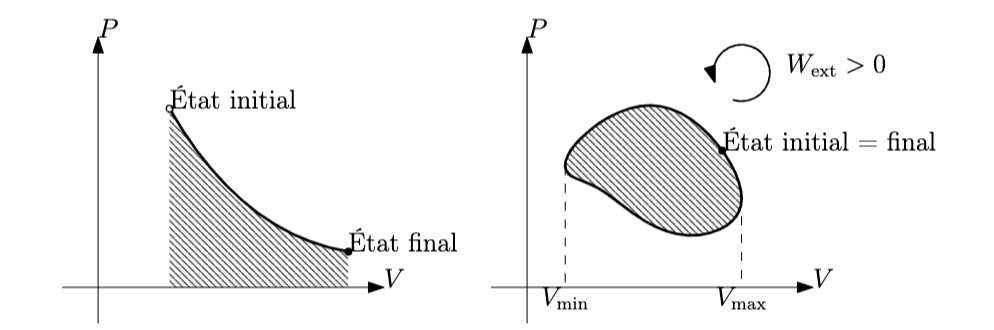
\includegraphics[width=0.8\textwidth]{./assets/Travail des forces de pression.png}
  \caption{Travail des forces de pression}
  \label{fig:Travail des forces de pression}
\end{figure}


Explication : Si $\delta W >0$, le système reçoit du travail, i.e. $\mathrm{d}V < 0$ car le système subit une compression. Sinon, le système subit une détente.
% subsection Travail algébrique reçu (end)

\subsection{Transfert thermique : Chaleur reçu} % (fold)
\label{sub:Transfert thermique : Chaleur reçu}

Le travail que l’extérieur exerce sur le système ne se limite pas au travail macroscopique décrit précédemment. Il existe également les interactions entre les très nombreux atomes du milieu extérieur et ceux de notre système ($\Sigma$), au niveau microscopique. Ces interactions, et leur travail, sont très complexes et il est impossible de les calculer ou de les mesurer directement à partir de données macroscopiques. Pourtant, elles contribuent aussi à la variation de l’énergie mécanique totale du système. 

Nous appelerons cet apport : le \textbf{transfert thermique} ou la \textbf{chaleur}.
% subsection Transfert thermique : Chaleur reçu (end)

\subsection{Énoncé} % (fold)
\label{sub:Énoncé}

\begin{Theorem}{Premier principe de la thermodynamique}{}
Les variations d'énergie mécanique d'un système fermé sont dues seulement au :
\begin{itemize}

    \item travail reçu 
    \item tranfert thermique reçu

\end{itemize}

\begin{equation}
  \Delta E _{tot} = [E _{c,\text{macro} } + U] _i ^{f} = W _{ext} + Q _{ext}
\end{equation}
\end{Theorem}

\subsection{Applications} % (fold)
\label{sub:Applications}

\begin{itemize}

    \item Transformation adiabatique : $Q = 0$ donc $\Delta U = W$ 
    \item Transformation isochore $\mathrm{d} U = 0$ donc $W = 0$, par conséquent $\Delta U = Q$
    \item Transformation monobare : utilisons l'\textbf{enthalpie}, $\Delta H = \Delta (U+PV) = Q$

\end{itemize}
% subsection Applications (end)


% subsection Énoncé (end)

% section Premier Principe de la thermodynamique (end)
% chapter Premier Principe de la thermodynamique (end)

\newpage
\section{Transformations Typiques} % (fold)
\label{sec:Transformations Typiques}

\subsection{Calorimétrie} % (fold)
\label{sub:Calorimétrie}

La méthode : 
\begin{itemize}

    \item Système étudié subit une transformation monobare : $Q = \Delta H$ 
    \item Système thermiquement isolé : $Q = 0$ 
    \item Équation : 
      \begin{equation}
        \sum_{i}^{} \Delta H_i = \Delta H _{\text{eau}} + \Delta H _{\text{calori}} + \dots = 0
      \end{equation}

\end{itemize}
% subsection Calorimétrie (end)
\subsection{Détente de Joule-Gay-Lussac} % (fold)
\begin{figure}[H] %h:当前位置, t:顶部, b:底部, p:浮动页
  \centering
  \includegraphics[width=0.8\textwidth]{./assets/Détente de Joule-Gay-Lussac.png}
  \caption{Détente de Joule-Gay-Lussac}
\end{figure}

On procède par :
\begin{itemize}
    \item Système au repos : $W = 0$, calorifugé : $Q = 0$
    \item Premier principe : $[U] _i ^{f}= 0$ 
    \item Gaz parfait : $U(T_i) = U(T_f)$ donc $T_i = T_f$ 


\end{itemize}

\subsection{Détente de Joule-Thomson} % (fold)
\label{sub:Détente de Joule-Thomson}

\begin{figure}[H] %h:当前位置, t:顶部, b:底部, p:浮动页
  \centering
  \includegraphics[width=0.8\textwidth]{./assets/Détente de Joule-Thomson.png}
  \caption{Détente de Joule-Thomson}
  \label{fig:Détente de Joule-Thomson}
\end{figure}

La détente de Joule-Thomson : 
\begin{itemize}

    \item fluide s'écoule très lentement 
    \item pression différente : $P_e > P_s$
    \item Régime permenant
    \item Parois calorifugée

\end{itemize}

On analyse : 
\begin{itemize}

    \item Premier principe :
      \begin{equation}
        [E _{c, \text{macro}} + U] _t ^{t + \mathrm{d}t} = W _{ext}
      \end{equation}

    \item Travail : 
      \begin{equation}
        W _{ext} = P_e V _{A A'} - P_s V _{B B'}
      \end{equation}

    \item En RP, énergie interne : 
      \begin{equation}
        [U]_t ^{t + \mathrm{d}t} = U _{BB'} - U _{A A'}
      \end{equation}

    \item De même pour l'énergie cinétique (macroscopique)
    \item La masse reste inchangée, car le système est fermé : 
      \begin{equation}
        M _{A A'} = M _{B B'}
      \end{equation}
    \item Le bilan d'énergie : 
      \begin{equation}
        \frac{E _{c, \text{macro}, A A'}}{M _{A A'}}  + \frac{U + P_e  V _{A A'}}{M _{A A'}}  = 
        \frac{E _{c, \text{macro}, BB'}}{M _{BB'}}  + \frac{U + P_s V _{BB'}}{M _{BB'}}   
      \end{equation}

    \item Donc, 
      \begin{equation}
        \frac{v_e ^{2}}{2}  + h_e = \frac{v_s ^{2}}{2}  + h_s
      \end{equation}

    \item Variation d'énergie cinétique massique est négligeable, donc nous aurons 
      \begin{equation}
        h_e = h_s
      \end{equation}
      conservation de l'enthalpie massique. De même, elle ne fait pas varier sa température.
\end{itemize}





% subsection Détente de Joule-Thomson (end)

\subsection{Transformation adiabatique quasi-statique : Loi de Laplace} % (fold)
\label{sub:Transformation adiabatique quasi-statique}

\begin{figure}[H] %h:当前位置, t:顶部, b:底部, p:浮动页
  \centering
  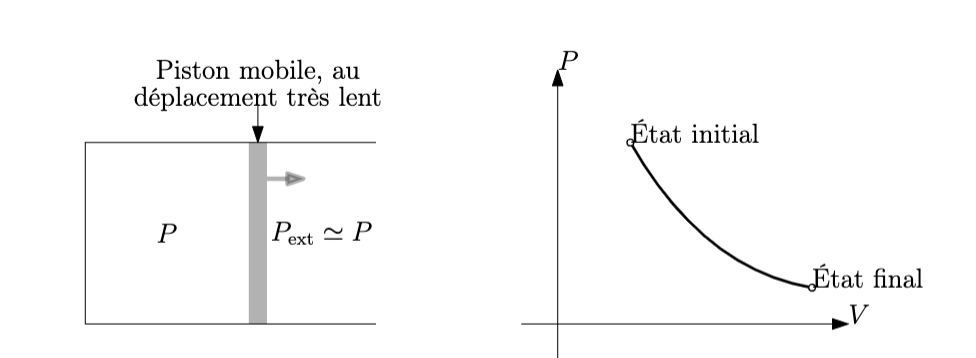
\includegraphics[width=0.8\textwidth]{./assets/Transformation adiabatique quasi-statique d'un gaz parfait.png}
  \caption{Transformation adiabatique quasi-statique d'un gaz parfait}
  \label{fig:Transformation adiabatique quasi-statique d'un gaz parfait}
\end{figure}

On procède comme :
\begin{itemize}

    \item Premier Principe : 
      \begin{equation}
        [U] _t ^{t + \mathrm{d}t} = - p \mathrm{d}V
      \end{equation}

    \item Propriété d'un gaz parfait : 
      \begin{equation}
        \mathrm{d} U = C_V \mathrm{d}T
      \end{equation}

    \item Par ailleurs 
      \begin{equation}
        T = \frac{PV}{nR}  \implies \mathrm{d}T = \frac{1}{nR} (p \mathrm{d}V + V \mathrm{d}p)
      \end{equation}

    \item Enfin, 
      \begin{equation}
        C_v \mathrm{d}T = - p \mathrm{d}V \implies \boxed{\frac{\mathrm{d}p}{p}  + \gamma \frac{\mathrm{d}V}{V} = 0}
      \end{equation}

    \item Ensuite, 
      \begin{equation}
       \mathrm{d} \ln (PV ^{\gamma}) = 0 \implies PV ^{\gamma} = \text{cte}
      \end{equation}


    
\end{itemize}

    On obtient :
    \begin{Theorem}{
        Loi de Laplace : transformation adiabatique quasi-statique
      }{}
    \begin{equation}
      PV ^\gamma = \text{cte}, \quad TV ^{\gamma-1} = \text{cte}, \quad P ^{1-\gamma} T ^\gamma = \text{cte}
    \end{equation}
    \end{Theorem}

% subsection Transformation adiabatique quasi-statique (end)

    \subsubsection{Conséquence du loi de Laplace} % (fold)
    \label{sec:Conséquence du loi de Laplace}
   \begin{Definition}[colbacktitle=red!75!black]{Coefficient de compressibilité isotherme}{}
   \begin{equation}
     \chi_T = - \frac{1}{V}  \left( \frac{\partial V}{\partial P}  \right)_T
   \end{equation}
   Pour une petite variation de $\Delta P$, on observe une changement : 
   \begin{equation}
     \Delta V = - \chi_T V_0 \Delta P
   \end{equation}
   \end{Definition}

   \begin{Definition}[colbacktitle=red!75!black]{
       Coefficient de compressibilité isentropique
     }{}
   \begin{equation}
     \chi_S = - \frac{1}{V}  \left( \frac{\partial V}{\partial P}  \right)_S
   \end{equation}
   \end{Definition}

   
   Pour un gaz parfait : 
   \begin{itemize}

       \item isotherme : 
         \begin{equation}
           PV = nRT= \text{cte} \implies V = \frac{P_0 V_0}{P}         
         \end{equation}

       \item isentropique : 
         \begin{equation}
           PV ^{\gamma} = \text{cte} \implies V = \frac{P_0 ^{1/ \gamma}V_0}{P ^{1/\gamma}} 
         \end{equation}

        \item On a toujours 
          \begin{equation}
            \chi_T = \gamma \chi_S
          \end{equation}

   \end{itemize}

    
    % subsubsection Conséquence du loi de Laplace (end)


% subsection D'etente de Joule-Gay-Lussac (end)
% section Transformations Typiques (end)
